\documentclass[12pt]{article}

\usepackage{polski}
\usepackage[utf8]{inputenc}
\usepackage{graphicx} 
\usepackage{hyperref}
\hypersetup{pdftex, colorlinks=true, allcolors=blue}
\usepackage{hypcap}
\usepackage{pdfpages}

\title{Dokumentacja - Gra "Statki kosmiczne"}
\author{Ernest Bieś, Konrad Czechowski, Dawid Kwaśny}
\begin{document}
\maketitle
\tableofcontents
\newpage
\section{Podstawowe informacje}
"Statki kosmiczne" to gra logiczna będąca połączeniem dwóch popularnych gier "Statki" oraz "Saper". \\

\section{Zasady gry}
Po rozpoczęciu gry na planszy o wymiarach 9x9 utworzonej z kwadratów są losowo rozmieszczone statki kosmiczne o różnych wielkościach:\\
Dwa \textit{Transportowce} o wymiarze 4\\
Trzy \textit{Samoloty kosmiczne} o wymiarze 3\\
Trzy \textit{Wahadłowce} o wymiarze 2\\
Dwa \textit{Szturmowce} o wymiarze 1\\
\\
Statki nie są widoczne. Zadaniem gracza jest odnalezienie wszystkich statków w jak najmniejszej liczbie kroków. W przypadku odkrycia pola, które nie zawiera żadnego statku widoczna jest liczba, która wskazuje na ilu polach sąsiadujących z odkrytym polem znajdują się statki. Wobec powyższego gracz musi podejmować swoją decyzję dotyczącą pola, które w następnej kolejności odkryje na podstawie logicznego myślenia, gdyż tym samym zwiększa swoje szanse na odnalezienie statków w pobliżu.\\
\newpage
\begin{figure}[h]
\section{Opis klienta}
\subsection{Środowisko programistyczne}
Klient gry "Statki kosmiczne" został utworzony z wykorzystaniem darmowego środowiska programistycznego QtCreator 4.9.1.
\subsection{Interfejs graficzny klienta}
\centering
\includegraphics[width=12cm]g
\caption{Okno główne programu}
\end{figure}
W głównym oknie programu po lewej stronie widoczna jest plansza o rozmiarze 9x9 kwadratów na której wyświetlane są ikony zestrzelonych statków oraz pola, które zostały odkryte przez gracza, a nie zawierają żadnych statków. Po uruchomieniu gry po lewej stronie wyświetlone zostają podstawowe informacje dotyczące zasad gry oraz statków jakie musimy zestrzelić. W górnym lewym rogu znajduje się przycisk za pomocą którego możemy ukryć zasady gry. W lewym dolnym rogu okna znajdują się pola służące do wprowadzenia nazwy użytkownika i hasła oraz przyciski za pomocą których możemy utworzyć nową grę na serwerze lub wczytać już istniejącą.Na dole w srodku okna znajduje się konsola na której wyświetlane są informacje dotyczące akcji podejmowanych przez gracza. Z prawej strony w dolnej części okna znajduje się licznik z aktualnie wykonanymi krokami przez gracza.\\

\begin{figure}[h]
\centering
\includegraphics[width=12cm]b
\caption{Okno w trakcie gry}
\end{figure}
W trakcie gry użytkownik po wskazaniu myszką wybranego pola i naciśnięciu lewego przycisku myszki odsłania poszczególne pola na planszy. W przypadku trafienia statku jego ikona zostaje wyświetlona w odpowiednim miejscu na planszy, natomiast w przypadku "pudła" we wskazanym polu pojawia się znak X oraz liczba wskazująca na ilu polach sąsiadujących ze wskazanym znajdują się statki.Równocześnie po wskazaniu pola odtwarzany jest odpowiedni dźwięk.\\
\newpage
\subsection{Instrukcja obsługi}
Po uruchomieniu klienta użytkownik wprowadza nazwę użytkownika oraz hasło, a następnie naciska przycisk "Nowa gra". Zostaje utworzona nowa gra dla użytkownika, następnie korzystając z myszki naciska lewy przycisk na wybranym polu na planszy. Jeżeli pod odkrytym polem znajduje się statek, jego ikona zostanie wyświetlona w odpowiednim kwadracie oraz program zasygnalizuje trafienie odpowiednim dźwiękiem. Jeżeli natomiast wskazane pole nie zawiera żadnego statku to zostanie na nim wyświetlony znak X oraz liczba wskazująca na ilu polach sąsiadujących znajdują się statki. Jednocześnie za każdym wskazaniem pola zostaje zwiększony licznik znajdujący się w prawym, dolnym roku ekranu. Jednocześnie na konsoli będą pojawiały się komunikaty dotyczące trafienia danego statku, jego nazwy lub też, że oddany strzał to niestety "pudło".\\
Po zestrzeleniu wszystkich statków kosmicznych wyświetlany jest komunikat z zapytaniem czy użytkownik chce zakończyć działanie programu. W przypadku udzielenia negatywnej odpowiedzi gra jest zapisywana na serwerze, natomiast klient zeruje wszelkie dane i ustawienia celem umożliwienia użytkownikowi rozpoczęcia nowej gry.
\begin{figure}[h]
\centering
\includegraphics[width=11cm]k
\caption{Okno po zakończeniu gry}
\end{figure}

\section{Analiza problemu}

\section{Implementacja}
\includepdf[pages=13-21,pagecommand={}]{../Doxygen/latex/refman.pdf}

\section{Testowanie}
\section{Proponowane dalsze możliwości rozbudowy}

\section{Instrukcja kompilacji}
Oprócz standardowej kompilacji z poziomu środowiska QtCreator możemy skompilować program ręcznie. Poleceniem \textit{qmake} należy wygenerować plik Makefile. Następnie wystarczy uruchomić polecenie \textit{make}, a po chwili w katalogu pojawi się skompilowany plik wykonywalny.

\end{document}
